\documentclass[dvipdfmx, 10.5pt]{beamer}
%%%% 和文用 %%%%%
\usepackage{bxdpx-beamer}
\usepackage{pxjahyper}
\usepackage{minijs}%和文用
\renewcommand{\kanjifamilydefault}{\gtdefault}%和文用
\usepackage{comment} %コメントアウト用

%%%%%%%%%%%%%%%%%%%%%%%%%%
%% usepackage 群
%%%%%%%%%%%%%%%%%%%%%%%%%%
\usepackage{amsmath,bm} %多次元空間ベクトルRを表記するのに必要
\usepackage{amsfonts}
\usepackage{ascmac} %枠付き文章を表記するのに必要
\usepackage{amssymb}
% \usepackage[dvipdfmx]{animate} %アニメーション
% \usepackage[dvipdfmx]{graphicx} %画像挿入
% \mathbb{R}^{l} %表記例
\usepackage{algorithm}
% \usepackage{algorithmicx}
\usepackage{algpseudocode}
\usepackage{animate} %アニメーション

%%%%%%%%%%%%%%%%%%%%%%%%%%
%% bibtex 群
%%%%%%%%%%%%%%%%%%%%%%%%%%
% biblatex.標準のバックエンドはbiber
%\usepackage{biblatex}
% bibtexのファイル
% \addbibresource{mybib.bib}
% 参考文献のインデックスを文字列で表示
% \setbeamertemplate{bibliography item}[text]

%%%%%%%%%%%%%%%%%%%%%%%%%%
%% tikz 群
%%%%%%%%%%%%%%%%%%%%%%%%%%
\usepackage{tikz}
\usetikzlibrary{positioning}

\usetikzlibrary{calc, intersections, arrows, math}
\usetikzlibrary{arrows, positioning, shapes.callouts}
\usetikzlibrary{decorations,decorations.pathreplacing}

\graphicspath{{./fig/}}

%%%% スライドの見た目 %%%%%
\usetheme{Madrid}
\usefonttheme{professionalfonts}

%%%% metropolisの設定 %%%%%
% \metroset{block=fill}


%\useoutertheme[subsection=false]{smoothbars}%ヘッダーにセクション表示
\useinnertheme{circles} % 箇条書きをシンプルに

\setbeamercovered{transparent}%消えている文字をうっすらと表示
\setbeamertemplate{footline}[frame number]%フッターをページ番号だけに
\setbeamerfont{footline}{size=\scriptsize}%ページ番号小さく
\setbeamerfont{frametitle}{size=\large}%フレームタイトルちょい小さく
\setbeamercolor{footline}{bg=black}%ページ番号を太く
\setbeamersize{text margin left=.75zw, text margin right=.75zw}%スライドの横の空白を調節
% \setbeamertemplate{itemize item}{\small\raise0.5pt\hbox{$\bullet$}}
\setbeamertemplate{itemize subitem}{\scriptsize\raise1.5pt\hbox{$\blacktriangleright$}}
\setbeamertemplate{itemize subsubitem}{\scriptsize\raise1.5pt\hbox{$\bigstar$}}

\setbeamertemplate{enumerate items}[default]%enumerate環境のitemを見やすくする
\setbeamertemplate{section in toc}[square]%outlineのボールを四角に
\setbeamertemplate{navigation symbols}{}%右下のアイコンを消す

% blockの色定義
\definecolor{BlueTOL}{HTML}{222288}
\definecolor{BrownTOL}{HTML}{666633}
\definecolor{GreenTOL}{HTML}{228822}
\definecolor{RedTOL}{HTML}{882222}

\setbeamercolor{block title}{fg=white, bg=BlueTOL}
\setbeamercolor{block body}{fg=black, bg=BlueTOL!10!white}
\setbeamercolor{block title alerted}{fg=white, bg=RedTOL}
\setbeamercolor{block body alerted}{fg=black, bg=RedTOL!10!white}
\setbeamercolor{block title example}{fg=white, bg=GreenTOL}
\setbeamercolor{block body example}{fg=black, bg=GreenTOL!10!white}

%%%%

%%%%%%%%%%%%%%%%%%%%%%%%%%%%%%%%%%%%%%%%%%%%
%%いろいろ便利なもの
%%%%%%%%%%%%%%%%%%%%%%%%%%%%%%%%%%%%%%%%%%%%
\usepackage{here} %[hbtp]の代わりに[H]と書きこむと強制的にその場所に図や表を挿入する
\usepackage{bm}
\usepackage{amsmath}

%%%%%%%%%%%%%%%%%%%%%%%%%%%%%%%%%%%%%%%%%%%%%%%%%
%%newcommand群
%%%%%%%%%%%%%%%%%%%%%%%%%%%%%%%%%%%%%%%%%%%%%%%%%
\newcommand{\argmax}{\mathop{\rm arg~max}\limits}
\newcommand{\argmin}{\mathop{\rm arg~min}\limits}

\newcommand{\EE}{{\mathbb E}} % 期待値のE (追加)
\newcommand{\cN}{{\cal N}}
% \newcommand{\a}{\bm{a}}
% \newcommand{\b}{\bm{b}}
% \newcommand{\c}{\bm{c}}
% \newcommand{\d}{\bm{d}}
% \newcommand{\e}{\bm{e}}
% \newcommand{\f}{\bm{f}}
% \newcommand{\g}{\bm{g}}
% \newcommand{\h}{\bm{h}}
% \newcommand{\i}{\bm{i}}
% \newcommand{\j}{\bm{j}}
% \newcommand{\k}{\bm{k}}
% \newcommand{\l}{\bm{l}}
% \newcommand{\m}{\bm{m}}
% \newcommand{\n}{\bm{n}}
% \newcommand{\o}{\bm{o}}
% \newcommand{\p}{\bm{p}}
% \newcommand{\q}{\bm{q}}
% \newcommand{\r}{\bm{r}}
% \newcommand{\s}{\bm{s}}
% \newcommand{\t}{\bm{t}}
% \newcommand{\u}{\bm{u}}
% \newcommand{\v}{\bm{v}}
% \newcommand{\w}{\bm{w}}
% \newcommand{\x}{\bm{x}}
% \newcommand{\y}{\bm{y}}
% \newcommand{\z}{\bm{z}}
\newcommand{\ul}{\underline}
\newcommand{\us}{\underset}

\newcommand{\zl}{\rightarrow}
\newcommand{\zh}{\leftarrow}

%%%%%%%%%%%%%%%%%%%%%%%%%%%%%%%%%%%%%%%%%%%%%%%%%
%%追加
%%%%%%%%%%%%%%%%%%%%%%%%%%%%%%%%%%%%%%%%%%%%%%%%%
\renewcommand{\algorithmicrequire}{\textbf{Input:}}


%%%%%%%%%%%%%%%%%%%%%%%%%%%%%%%%%%%%%%%%%%%%%%%%%
%%本文
%%%%%%%%%%%%%%%%%%%%%%%%%%%%%%%%%%%%%%%%%%%%%%%%%
\title[]{Gaussian Process Optimization in the Bandit Setting:\\No Regret and Experimental Design}
\subtitle{}
\author[]{Niranjan Srinivas, Andreas Krause$^{\dag}$, Sham Kakade$^{\dag\dag}$, Matthias Seeger$^{\dag\dag\dag}$}
\date[\today]{\today}
\institute[]{$\dag$: California Institute of Technology\\
$\dag\dag$: University of Pennsylvania\\
$\dag\dag\dag$: Saarland University}
% [..]に省略名が書ける

%目次スライド
\AtBeginSection[noframenumbering]{
    \begin{frame}[noframenumbering]{Next Section}
	\tableofcontents[currentsection, hidesubsections]%目次本体
	\thispagestyle{empty}%ヘッダーフッター表示なし
	\end{frame}
}

\begin{document}

%-------------------

%タイトル
\begin{frame}[plain, noframenumbering]
\maketitle%タイトル本体
\thispagestyle{empty}%ヘッダーフッター表示なし
% \addtocounter{framenumber}{-1}%ページ数カウンタしない
\end{frame}

%-------------------


%目次
\begin{frame}[noframenumbering]{目次}
	\tableofcontents[hideallsubsections]
	\thispagestyle{empty} %ページ番号なし
\end{frame}

%-------------------
\section{はじめに}
%-------------------

\subsection{背景}
\begin{frame}{\insertsubsection}
	\begin{itemize}
		\item 多くの実問題は目的関数に対する最適変数探索問題として定式化できる
		\begin{itemize}
			\item 耐久性の高いロボットの開発
		\end{itemize}
	\end{itemize}
	\begin{center}
		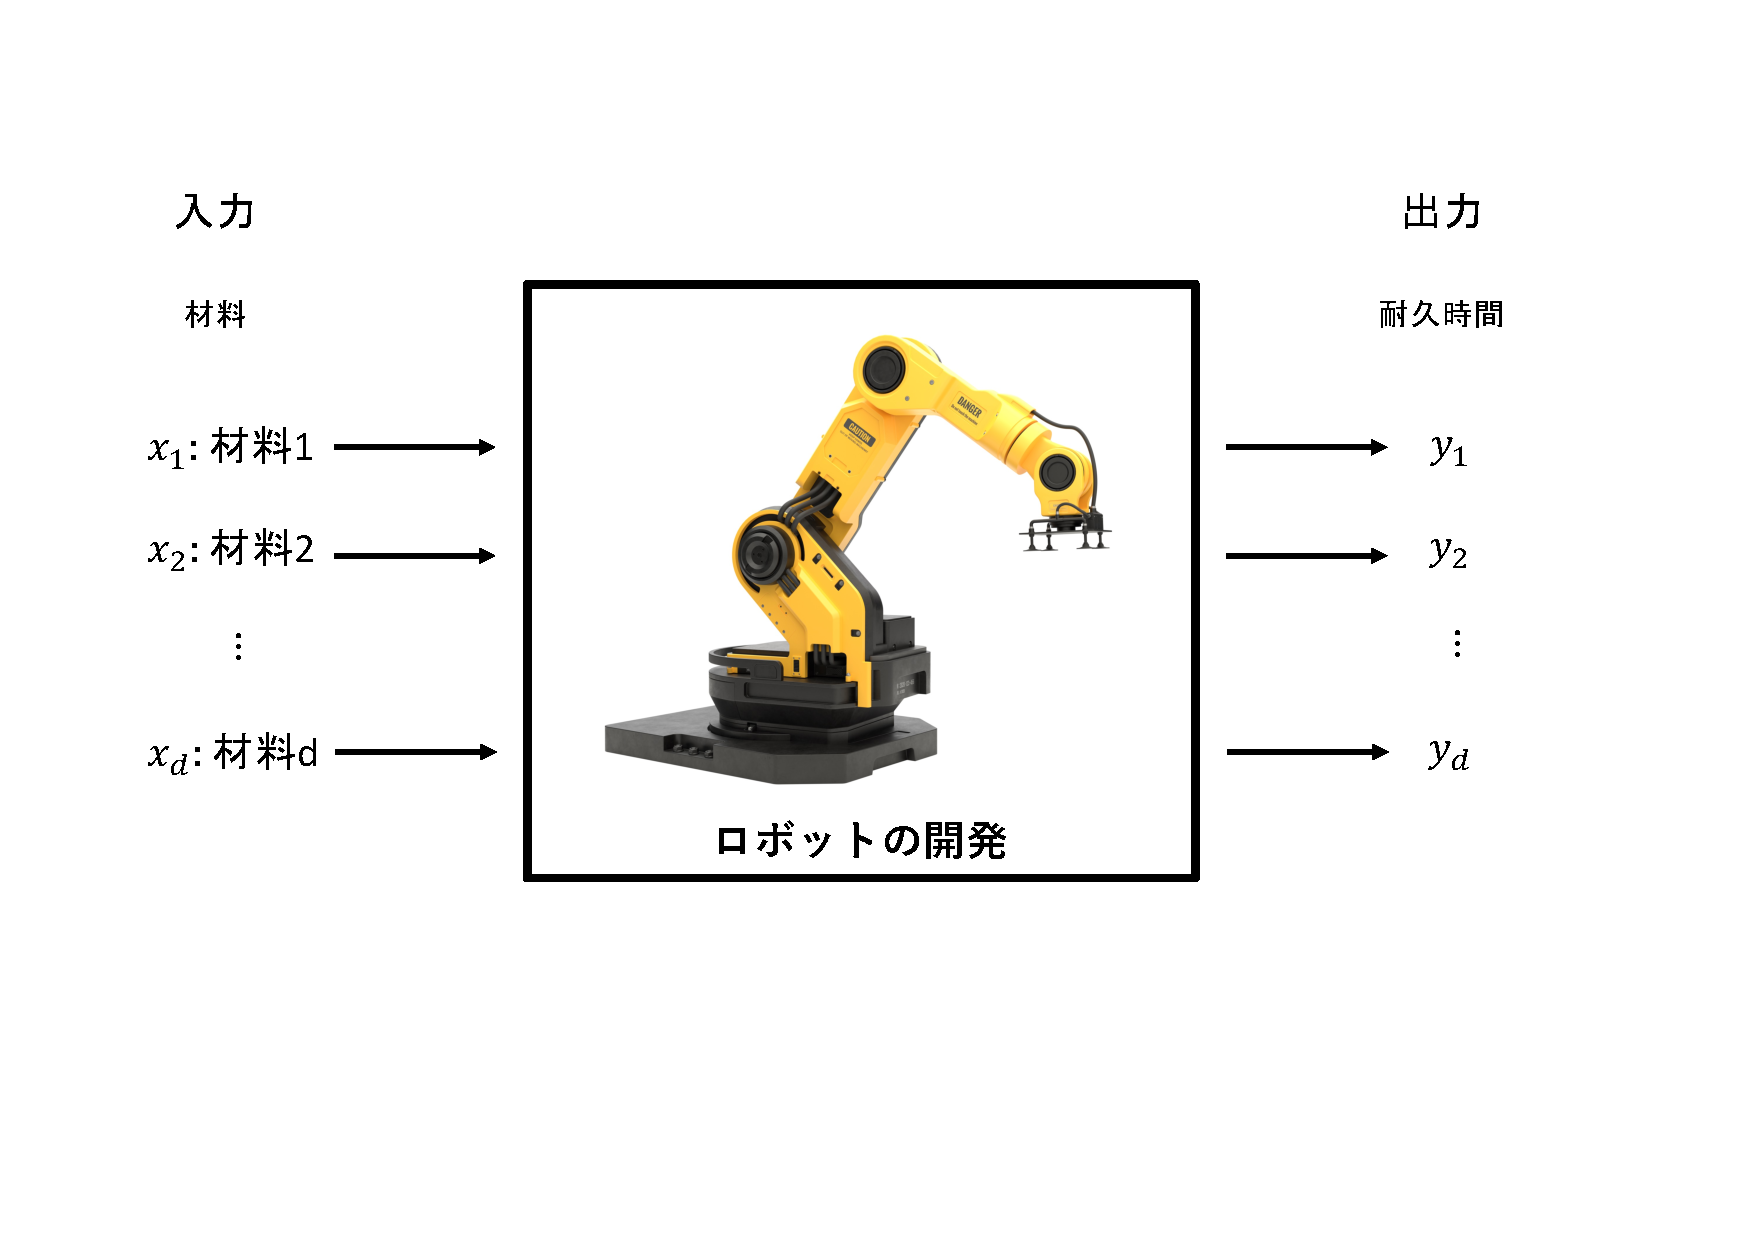
\includegraphics[width=0.80\textwidth]{./Fig/Robot.pdf}
	\end{center}
\end{frame}

%-------------------



\subsection{ブラックボックス関数}
\begin{frame}{\insertsubsection}
	\begin{itemize}
		\item ブラックボックス関数 $f$
		\begin{align*}
			y_i = f(\bm x_i) + \varepsilon_i
		\end{align*}
		\begin{center}
			入力:$\bm x_i$,\quad
			出力:$y_i$,\quad
			誤差:$\varepsilon_i$
		\end{center}
	\end{itemize}

	\begin{center}
		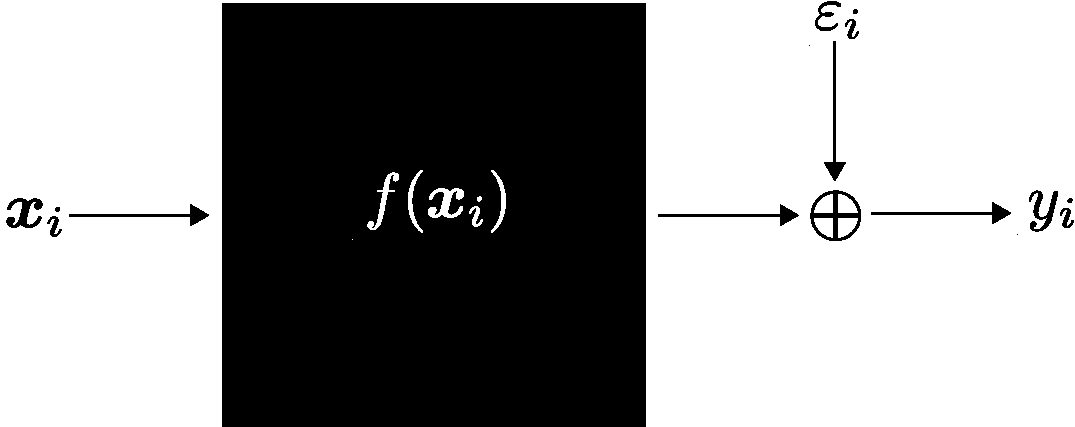
\includegraphics[width=0.50\textwidth]{./Fig/blackbox.pdf}
	\end{center}

	\begin{itemize}
		\item 実応用で扱う対象はブラックボックス関数であることが多い
		\item ブラックボックス関数は具体的な形状が不明

	\end{itemize}
\end{frame}

%-------------------



\subsection{ベイズ最適化}
\begin{frame}{\insertsubsection}
%		\begin{itemize}
%			\item ベイズ最適化は,確率論的アプローチを用いた最適化手法である
%			\item そのため,不確実性を含む問題を解決するために用いられていることが多い
%			\item そのような問題を扱うために,事前分布を用いて事後分布を求めることができる
%			\item 論文中では,このようなベイズ最適化を用いて,ガウス過程を用いた最適化問題を解決するアルゴリズムを提案している.
%			\item また,そのアルゴリズムがバンディット設定でも有効であることを示している.
%		\end{itemize}
	\begin{center}
		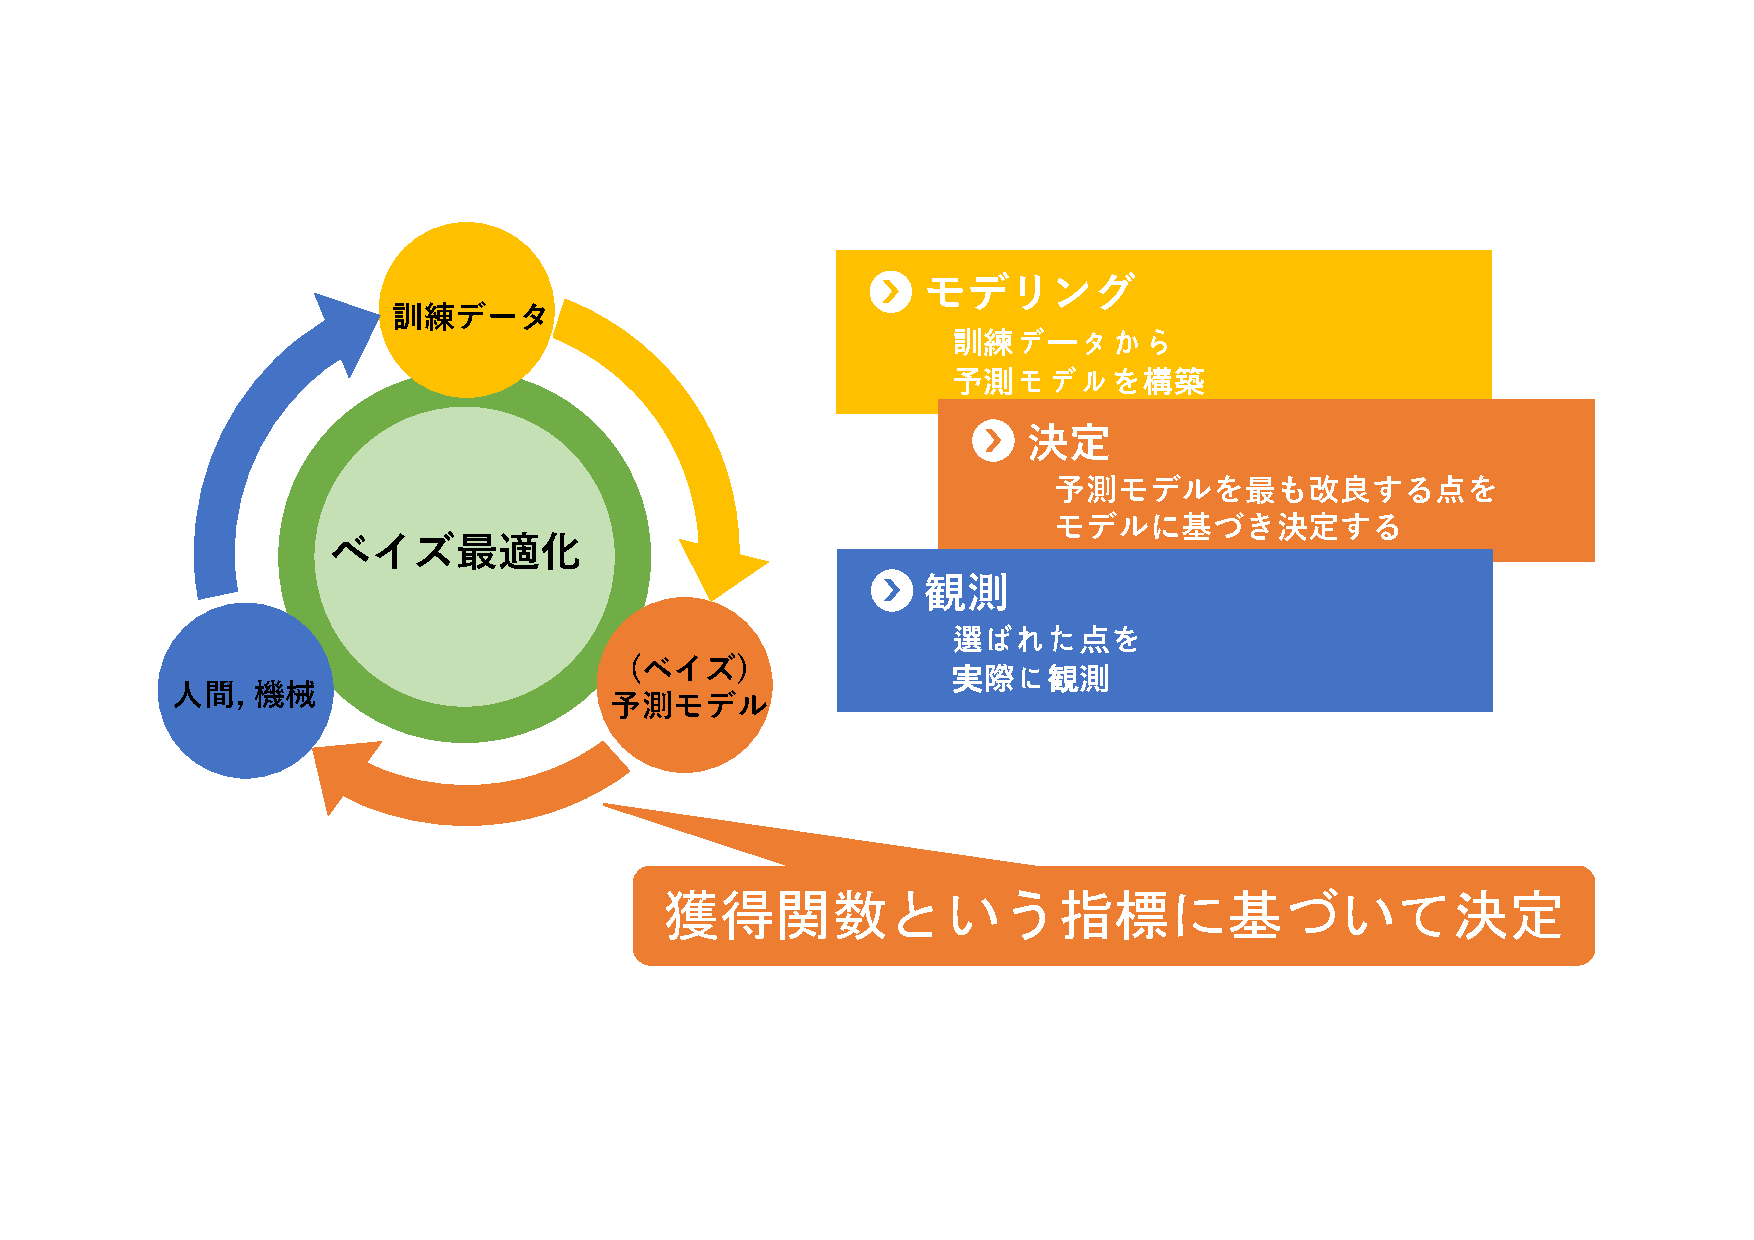
\includegraphics[width=0.80\textwidth]{./Fig/BO.pdf}
	\end{center}
	\begin{itemize}
		\item 多くの実問題はブラックボックス関数最適化と等価
		\item 各入力における関数値を得るには大きなコストがかかる
		\item できるだけ少ない関数評価回数で最適化を見つけたい
		\item 有効な手法として\alert{ベイズ最適化}がある
	\end{itemize}

\end{frame}

%-------------------

	% \subsection{バンディット問題}
	% \begin{frame}{\insertsubsection}
	% 	\begin{itemize}
	% 		\item 序論として,バンディット問題について説明する(前提知識の提供)
	% 		\begin{itemize}
	% 			\item バンディット設定とは,決定をする際に報酬を得ることができるが,そのためには,その決定をする前にその詳細を知ることができない設定を指す
	% 			\item このような設定では,報酬を最大化することを目的として,決定をする場所を最適に選択することが重要になる
	% 			\item バンディット問題の具体例:投資をする場合や,商品を購入する場合など.このような場面では,最適な決定をすることで,最大の報酬を得ることができるため,重要である.
	% 		\end{itemize}
	% 	\end{itemize}
	% \end{frame}


%-------------------

\subsection{本論文の貢献}

\begin{frame}{\insertsubsection}

		\begin{block}{貢献}
			\begin{itemize}
				\item ガウス過程を用いた最適化問題を解決するためのアルゴリズムを提案
				\item 実データ実験において優れた性能を発揮
			\end{itemize}
		\end{block}


		% \begin{itemize}
		% 	\item 計算機科学や統計学において,最適化問題は非常に重要であることを強調する
		% 	\item ガウス過程を用いた最適化は,複雑で非線形な関数を扱う場合に有用であることを紹介する
		% 	\item バンディット設定において,最適な決定をすることが重要であることを紹介する
		% 	\item 今までにバンディット設定でのガウス過程最適化については,リグレット制限が証明されていなかった
		% 	\item 本論文では,バンディット設定におけるガウス過程最適化において,リグレット制限を証明することで,最適な決定をするアルゴリズムを提案する
		% \end{itemize}

\end{frame}
%-------------------

%以降\sectionごとに目次表示
\section{ベイズ最適化}
%-------------------
% \subsection{ブラックボックス関数の定式化}
% \begin{frame}{\insertsubsection}
% 	\begin{itemize}
% 		\item[$\ast$] 本スライドでは,一章で述べたブラックボックス関数を定式化して説明する
% 		\item ブラックボックス関数
% 		\begin{align*}
% 			y_i = f(\bm x_i) + \varepsilon_i
% 		\end{align*}
% 		\begin{center}
% 			入力:$\bm x_i \in \mathcal{X} \subseteq \mathbb{R}^d$,\quad
% 			出力:$y_i \in \mathbb{R}$,\quad
% 			誤差:$\varepsilon_i \in \mathbb{R}$
% 		\end{center}
% 	\end{itemize}

% 	\begin{center}
% 		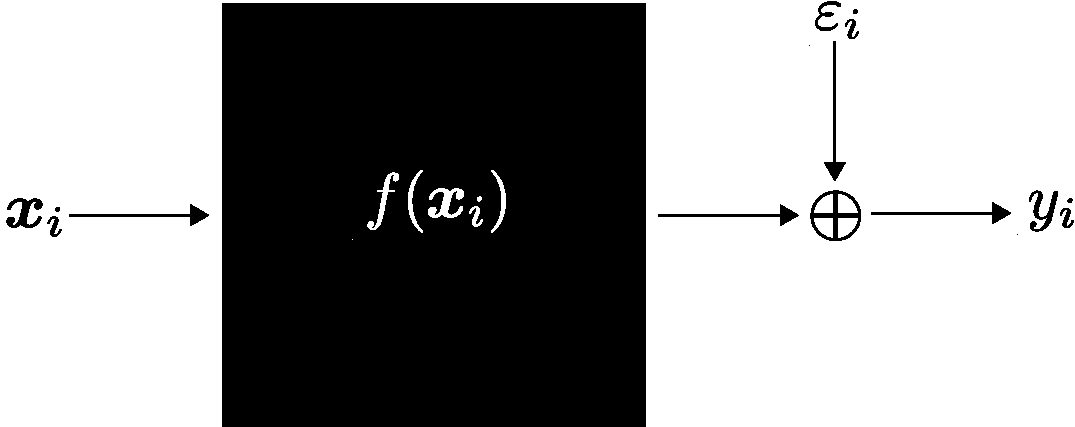
\includegraphics[width=0.80\textwidth]{./Fig/blackbox.pdf}
% 	\end{center}

% \end{frame}

%-------------------

\subsection{問題設定}
\begin{frame}{\insertsubsection}
	\begin{itemize}
		\item 候補入力$\mathcal{X} = \{ \bm x_1, \ldots, \bm x_n \}$が与えられている

		\item 関数$f$を評価して出力$y_i = f(\bm x_i)$を得るにはコストがかかる

		\item できるだけ少ないコストで関数$f$を最大化するパラメータ$\bm x$を求めたい
		\begin{align*}
			\bm x^* = \arg \max_{\bm x \in \mathcal{X}} ~ f(\bm x)
		\end{align*}
		\begin{itemize}
			\item ガウス過程は確率分布を用いた複雑で非線形な関数を扱うためのモデルである
			\item このような複雑で非線形な関数を扱う場合には一般的な最適化手法では解決が困難になることがある
		\end{itemize}
	\end{itemize}
\end{frame}

%-------------------

\subsection{ガウス過程}
\begin{frame}{\insertsubsection}
	\begin{block}{ガウス過程}
		任意の入力$\{ \bm x_1, \ldots, \bm x_n \}$に対して$\{f(\bm x_1), \ldots, f(\bm x_n)\}$がn次元正規分布に従うなら$f$はガウス過程に従う
	\end{block}

\begin{itemize}
	\item 関数$f$がガウス過程に従うことを$f(\bm x) \sim \mathcal{GP}(\mu(\bm x), k(\bm x, \bm x'))$
	\item 平均関数: $\mu(\bm x) = \mathbb{E}[f(\bm x)]$
	\item 共分散関数(カーネル関数): $k(\bm x, \bm x') = \mathbb{E}[(f(\bm x) - \mu(\bm x))(f(\bm x') - \mu(\bm x'))]$
\end{itemize}
\end{frame}

%-------------------


\subsection{ガウス過程を用いたベイズ最適化}
\begin{frame}{\insertsubsection}
	\begin{itemize}
		\item $f$にガウス過程事前分布$\mathcal{GP}(0, k(\bm x, \bm x'))$を仮定する
		\item 訓練データ$(X, \bm y) = \left\{ (\bm x_i, y_i) \right\}_{i=1}^t$に基づき$f$の事後分布を求める
		\item 事後分布に基づき\alert{最適な点}を次に観測する
		\item 観測した$(x_{next}, y_{next})$を訓練データに追加し再び事後分布を求める
	\end{itemize}
	\begin{align*}
		f({\bm x}_\ast) \mid \mathcal{D}
		 \sim
		 N \left(
		 \underbrace{
		 \bm k_{\mathcal{D}, {\bm x}_\ast   }^\top
		 K_{\mathcal{D} \mathcal{D}}^{-1}
		 {\bm y}}_{\text{posterior mean}},
		 \underbrace{
		 k_{{\bm x}_\ast {\bm x}_\ast}
		 -
		 \bm k_{\mathcal{D} , {\bm x}_\ast}^\top
		 K_{\mathcal{D} \mathcal{D}}^{-1}
		 \bm k_{\mathcal{D} , {\bm x}_\ast}}_{\text{posterior variance}}
		 \right)
		\end{align*}

		\begin{tiny}
			\begin{align*}
			 \hspace*{-15mm}
			 K_{\mathcal{D} \mathcal{D}}
			 =
		\begin{pmatrix}
			 k(\bm x_{ 1}, \bm x_{ 1}) &
			 \cdots &
			 k(\bm x_{ 1}, \bm x_{ t}) \\
			 \vdots &
			 \ddots &
			 \vdots \\ 	 
			 k(\bm x_{ t}, \bm x_{ 1}) &
			 \cdots &
			 k(\bm x_{ t}, \bm x_{t}) 
		\end{pmatrix},
			 \bm k_{\mathcal{D} ,{\bm x}_\ast}
			 =
		\begin{pmatrix}
			 k(\bm x_{ 1}, \bm x_\ast) \\
			 \vdots \\
			 k(\bm x_{ t}, \bm x_\ast) 
		\end{pmatrix},
			 %
			 k_{{\bm x}_\ast, {\bm x}_\ast}
			 =
			 k(\bm x_{\ast}, \bm x_{\ast})
			\end{align*}
			\end{tiny}

\end{frame}

%-------------------


\subsection{獲得関数}
\begin{frame}{\insertsubsection}
	\begin{block}{獲得関数}
		探索する点を選択するために使用される関数 % \iffalse$\bm x_t$\fi, \iffalse$\alpha$\fi
	\end{block}
	\begin{itemize}
		\item 獲得関数をを$\alpha(\bm x_{t-1})$とすると次に観測する点$\bm x_t$は以下のように決定
	\end{itemize}
	\begin{align*}
		\bm x_t = \arg \max_{\bm x} ~ \alpha(\bm x_{t-1})
	\end{align*}
	\begin{block}{獲得関数の設計指針}
		活用と探索のバランスを考慮して設計する
	\end{block}
	\begin{itemize}
		\item 活用: 既知の領域を活用し既知の最適解を超える解を見つけること
		\item 探索: 未知の領域を探査し新たな最適解を見つけること
	\end{itemize}

\end{frame}

%-------------------


\subsection{従来の獲得関数}
\begin{frame}{\insertsubsection}
	\begin{block}{variance only}
		\begin{align*}
			\bm x_t = \arg \max_{\bm x} ~ \alert{\sigma}_{t-1}^{\alert{2}}(\bm x)
		\end{align*}
	\end{block}
	\begin{itemize}
		\item 予測分散が最大となる$\bm x$を選択
		\begin{itemize}
			\item[$\Rightarrow$] \alert{探索}中心
		\end{itemize}
	\end{itemize}
	\begin{block}{mean only}
		\begin{align*}
			\bm x_t = \arg \max_{\bm x} ~ \alert{\mu}_{t-1}(\bm x)
		\end{align*}
	\end{block}
	\begin{itemize}
		\item 予測平均が最大となる$\bm x$を選択
		\begin{itemize}
			\item[$\Rightarrow$] \alert{活用}中心
		\end{itemize}
	\end{itemize}
\end{frame}
%-------------------

\section{GP-UCB}
%-------------------

\subsection{提案手法}

\begin{frame}{\insertsubsection}
	\begin{itemize}
		\item 探索・活用に特化した手法では最適化がうまくいかない場合が多い
		\begin{itemize}
			\item[$\Rightarrow$] 探索と活用のバランスが取れるような手法を提案
		\end{itemize}
	\end{itemize}
	\begin{block}{GP-UCB: Gaussian Process Upper Confidence Bound}
		\begin{align*}
			\bm x_t = \arg \max_{\bm x \in \mathcal{D}} ~ \mu_{t-1}(\bm x) + \beta_t^{1/2} \sigma_{t-1}(\bm x).
		\end{align*}
	\end{block}
	\begin{itemize}
		\item $\beta_t$は,探索の度合いを表す定数
		\begin{itemize}
			\item $\beta_t$が小さい $\Rightarrow$ 予測平均の比重が大きくなる $\Rightarrow$ 活用重視
			\item $\beta_t$が大きい $\Rightarrow$ 予測分散の比重が大きくなる $\Rightarrow$ 探索重視
		\end{itemize}
	\end{itemize}

\end{frame}
%-------------------

\subsection{GP-UCBのアルゴリズム}
\begin{frame}{\insertsubsection}
\begin{algorithm}[H]
	\caption{The GP-UCB algorithm.}
	\label{alg:gpucb}
	\begin{algorithmic}
		\Require Input space $\mathcal{D}$; GP Prior $\mu_0 = 0$, $\sigma_0$, $k$
		\For{\texttt{$t = 1, 2,\ldots $}}			\State Choose $\bm x_t = \arg \max_{\bm x \in \mathcal{D}} ~ \mu_{t-1}(\bm x) + \sqrt{\beta_t} \sigma_{t-1}(\bm x)$
			\State Sample $y_t \gets f(\bm x_t) + \varepsilon_t$
			\State Perform Bayesian update to obtaion $\mu_t$ and $\sigma_t$
		\EndFor
	\end{algorithmic}
\end{algorithm}




\end{frame}

%-------------------

\section{実験}
%-------------------



\subsection{実験手法}
\begin{frame}{\insertsubsection}
	\begin{itemize}
		\item 実験手法
		\begin{itemize}
			\item variance only
			\item maximum mean
			\item Expected Improvement(EI)
			\item Most Probable Improvement(MPI)
			\item GP-UCB
		\end{itemize}
		\item \alert{Mean Average Regret} を用いた評価
		\begin{itemize}
			\item Regret = (真の関数の最大値) - (観測済みデータの最大値)
			\item Average Regret : 1回の試行中のRegretの平均
			\item Mean Average Regret : 全試行のAverage Regretの平均
		\end{itemize}
	\end{itemize}
\end{frame}

%-------------------
\subsection{実験対象データ}
\begin{frame}{\insertsubsection}
	\begin{enumerate}
		\item 合成データ
		\begin{itemize}
			\item $\mathcal{D} \in [0,1]$の範囲を一様に1000点で区切った点を候補点とする
			\item $T = 1000$, $\sigma^2 = 0.025$, $\delta = 0.1$
			\item 30回試行
		\end{itemize}
		\item 温度データ
		\begin{itemize}
			\item 46個のセンサーから1分間隔で5日以上計測された気温
			\item $T = 46$, $\sigma^2 = 0.5$, $\delta = 0.1$
			\item 2000回試行
		\end{itemize}
		\item 交通データ
		\begin{itemize}
			\item 357個のセンサーから1ヶ月間午前6時から午前までに通過する車の速度
			\item $T = 357$, $\sigma^2 = 4.78$, $\delta = 0.1$
		\end{itemize}
	\end{enumerate}
\end{frame}

%-------------------

\subsection{実験結果}

\begin{frame}{\insertsubsection}
	\begin{center}
		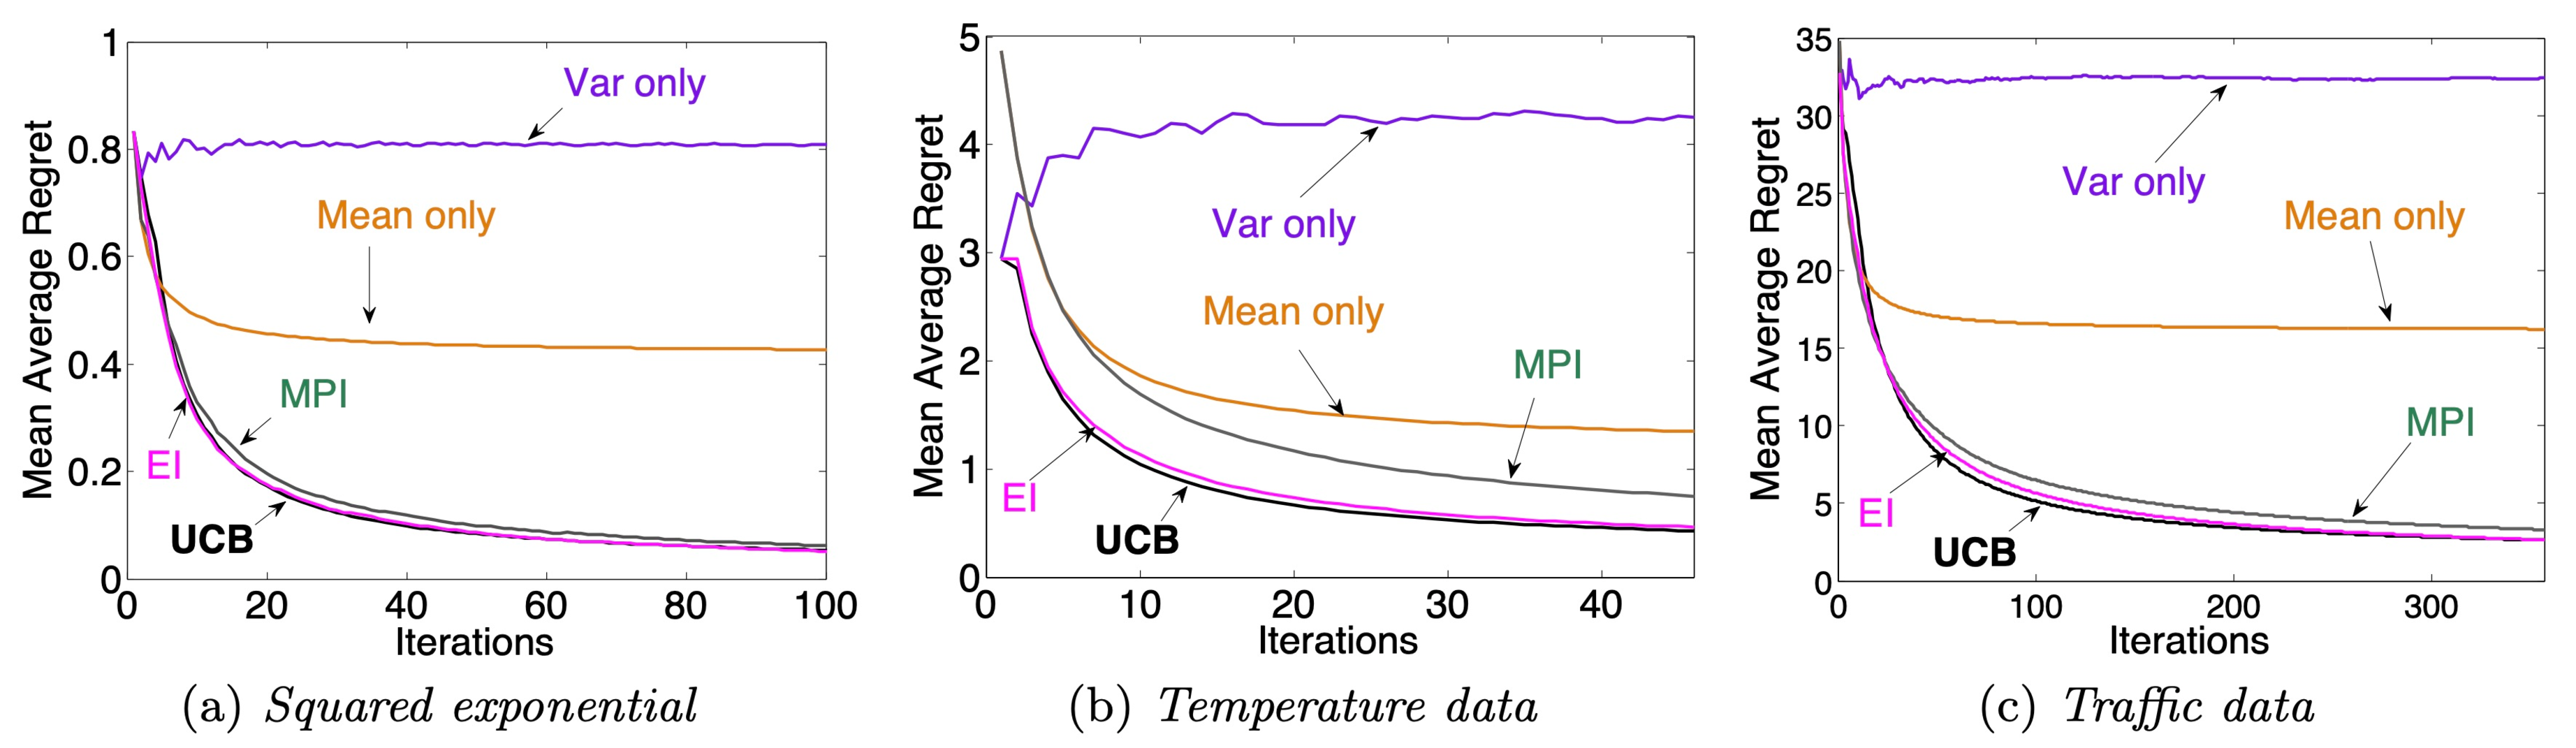
\includegraphics[width=0.90\textwidth]{./Fig/Figure4.pdf}
	\end{center}
	\begin{itemize}
		\item すべての実験結果においてGP-UCBが損失少なく最適化を行なっている
		\item 既存手法のEI,MPと比較して同等以上の性能を示した
	\end{itemize}

\end{frame}

%-------------------
\section{まとめ}

%-------------------

\subsection{結論}

\begin{frame}{\insertsubsection}
	\begin{itemize}
		\item GP-UCBというベイズ最適化の獲得関数を新たに提案
		\begin{itemize}
			\item GP-UCBは探索と活用を両立する獲得関数
		\end{itemize}
		\item GP-UCBは既存の手法と同等以上の性能を示した
		\begin{itemize}
			\item Mean Average Regretの観点で実データと合成データにおける性能を発揮
		\end{itemize}
		% \item We analyze GP-UCB, an intuitive algorithm for GP optimization, when the function is either sampled from a known GP, or has low RKHS norm.
		% \item We bound the cumulative regret for GP-UCB in terms of the information gain due to sampling, establishing a novel connection between experimental design and GP optimization.
		% \item By bounding the information gain for popular classes of kernels, we establish sublinear regret bounds for GP optimization for the first time. Our bounds depend on kernel choice and parameters in a fine-grained fashion.
		% \item We evaluate GP-UCB on sensor network data, demonstrating that it compares favorably to ex- isting algorithms for GP optimization.
	\end{itemize}

\end{frame}

%-------------------

% \subsection{まとめ2}
% \begin{frame}{\insertsubsection}
% 	\begin{itemize}
% 		\item テスト
% 	\end{itemize}

% \end{frame}

% %-------------------

\end{document}








